\chapter{Introdução} \label{ch:intro}

% Resumo opcional. Comentar se não usar.
\resumodocapitulo{"I never think of the future - it comes soon enough." - Albert Einstein}

% "I never think of the future - it comes soon enough." - Albert Einstein

\section{Contextualização}

Toda tecnologia surge no intento de reduzir o gasto de energia na execução de alguma tarefa. Nela consolidamos todo o conhecimento envolvido em alguma técnica permitindo a execução com um esforço muito menor a partir da consolidação disto em um objeto. A este damos diversos nomes: ferramentas, máquinas, robôs, lápis e caneta. Essencialmente todos com a mesma missão de permitir realizar qualquer tarefa a menor quantidade de energia possível.

As primeiras tecnologias utilizavam desta capacidade de executar as tarefas a partir de fenômenos naturais. Desta forma, o conhecimento aliado a propagação de calor do fogo, a fluidez da água e do vento e a rigidez da pedras nos permitiram conceber ferramentas cada vez mais complexas. Com o passar da história alcançamos o ponto dos próprios engenhos poderem ser iniciados e deixados a executarem tarefas sozinhos sem qualquer interferência de pessoas. No que então começamos a chamada automação.

% Citar alguma referência de história?
% Comentar um pouco sobre a história da automação
% História da robótica

%Dentre este universo novo de máquinas surge então o robô na tentativa replicar as capacidades humanas originadas em meio a evolução em um engenho que pude-se ser replicado e controlado. Em particular, replicar a capacidade de interagir com objetos de uma forma mais livre sem a necessidade de um completo estudo a respeito.

Robôs industriais, ou manipuladores robóticos, como também são chamados, se tornaram parte essencial na produção de bens aonde alguma das etapas exijam capacidades sobre-humanas de força, precisão, repetibilidade ou ainda na tolerância a altas temperatura e materiais corrosivos. Garantindo assim consistência, rapidez e segurança em tarefas de soldagem, montagem, pintura e corte no cenário industrial. No entanto, estas mesmas características que conferem a robustez apreciada no ambiente industrial tornam os robôs perigosos. A força, peso e velocidades de operação compõem elementos de risco na execução de atividades na presença de pessoas.

Mesmo sendo uma tecnologia bastante interessante na automação de processos que envolvam a manipulação de objetos, o uso de braços robóticos pode oferecer diversos riscos. Para garantir a segurança em ambiente industrial, diversas soluções são utilizadas como grades de isolamento, botões de parada e sistemas de detecção de pessoas. Atuando em geral na desativação do robô como forma de mitigar o risco.  No entanto para algumas atividade existe a necessidade da atuação conjunta de pessoas e máquinas. Para resolver este problema novos tipos de braços têm sido desenvolvidos incorporando características para segurança em cada aspecto do design, entre elas emprego de estruturas mais leves, operação em velocidades reduzidas, protocolos para interrupção em caso de acidentes e complacência.% \cite{nobody}

Ao que integra a categoria de robôs cooperativos, definidos pela norma  norma ISO/TS 15066:2016 \footnote{\url{https://www.iso.org/obp/ui/#iso:std:iso:ts:15066:ed-1:v1:en}}, como sistemas desenvolvidos para serem intrinsecamente seguros no uso em atividade em colaboração com pessoas. Por definição, são projetados para que seja oferecido o menor risco possível. Primeiro, estes robôs devem oferecer alguma forma de complacência, isto é deve ceder em caso de uma eventual colisão ou no por uma intenção diferente de movimento por parte de pessoas próximas evitando que a energia transmitida possa causar algum dano. Segundo, devem permitir operação em velocidades menores para reduzir o stress das pessoas na presença do robô. E com isto ainda ser capaz de executar a tarefa desejada. % Falta referência

Muito embora sempre exista a visão da tecnologia como vilã no roubo de empregos ao permitir ao uso de menos energia na execução de uma tarefa a redução do custo gera novas oportunidade por aumenta a capacidade de carga. Ainda que junto exista a necessidade de ressignificar o papel das pessoas no desenvolvimento de alguma atividade, deslocando o papel de total responsabilidade pela execução para incorporar papeis de planejamento pelo auxílio da automação, a incorporação de novas tecnologias traz um maior alcance dos produtos gerados. A partir do uso da tecnologia e da automação as pessoas migram do papel de agentes transformadores da matéria para agentes transformadores do processo permitindo que novos conhecimentos possam ser sempre incorporados.

% TODO Citar Referências do impacto do desenvolvimento tecnológico (ATM?)
% https://voxeu.org/article/how-computer-automation-affects-occupations

% Garantir flexibilidade e precisão: Tenho que ensinar kung fu ao robô...

% Robótica Cooperativa
% https://medium.com/@abhasvc/ais-threat-to-society-is-scarier-than-trump-ff7e9d42ea74
% https://www.hhs.se/contentassets/c8f677a0c9974bde950e2cec2edc51a1/substitution-of-labor-final.pdf
% http://www.nivelco.com.ua/documents/technical%20publications%20docs/Nof%20S.Y.%20Springer%20Handbook%20of%20Automation,%20Springer,%202009.pdf
% https://www.osha.gov/dts/osta/otm/otm_iv/otm_iv_4.html

\subsection{Breve histórico}

% Comentar sobre a história dos Cobots
%Uma primeiras implementações de robôs colaborativos foi no auxílio na tarefa de elevar um carga na vertical para facilitar o transporte e posicionamento de peças na fabricação de carros. Trata-se de uma tarefa repetitiva, que envolve o transporte de peças pesadas mas que não é possível de ser feita utilizando robôs por envolver o posicionamento de duas partes rígidas com enorme variabilidade de posição entre si.

%% Foto Lifter 

%% Foto Porta

%Posteriormente

% COG
%Seguindo uma filosofia diferente surgiu COG ( figura \ref{fig:domorobot} ), um robô humanoide desenvolvido pelo MIT para interação com pessoas\cite{nobody}. Seu projeto foi concebido para avaliar o comportamento conjunto de várias tecnologias existentes na época para a interação com pessoas. Dentre estes sistemas estava o uso de Atuadores Série Elásticos propostos por Pratt \cite{pratt1995series} como uma forma de permitir complacência ao atuador em conjunto de controle de torque preciso. De igual forma, ao ser introduzido um componente passivo permite reduzir a necessidade de um extenso planejamento na execução da tarefa como ocorre com braços rígidos.

% Domo e uso de Atuador Série Elástico
Baseado no humanoide COG em humanoides anteriores, em 2004 foi desenvolvido por Aaron Edsinger e Jeff Weber o robô Domo, mostrado na figura \ref{fig:domorobot}. Em seu projeto foram incorporadas diversas características visando permitir segurança através do uso de juntas complacentes com percepção de força. Bem como características para uso contínuo do ponto de vista mecânico como o uso de atuadores série elásticos baseados em fuso de esferas, proteção de superaquecimento para os motores e modularização do design. Para o controle são utilizados DSP para cada uma das juntas do robô\cite{edsinger2004domo}.

\begin{figure}[H]
    \centering
    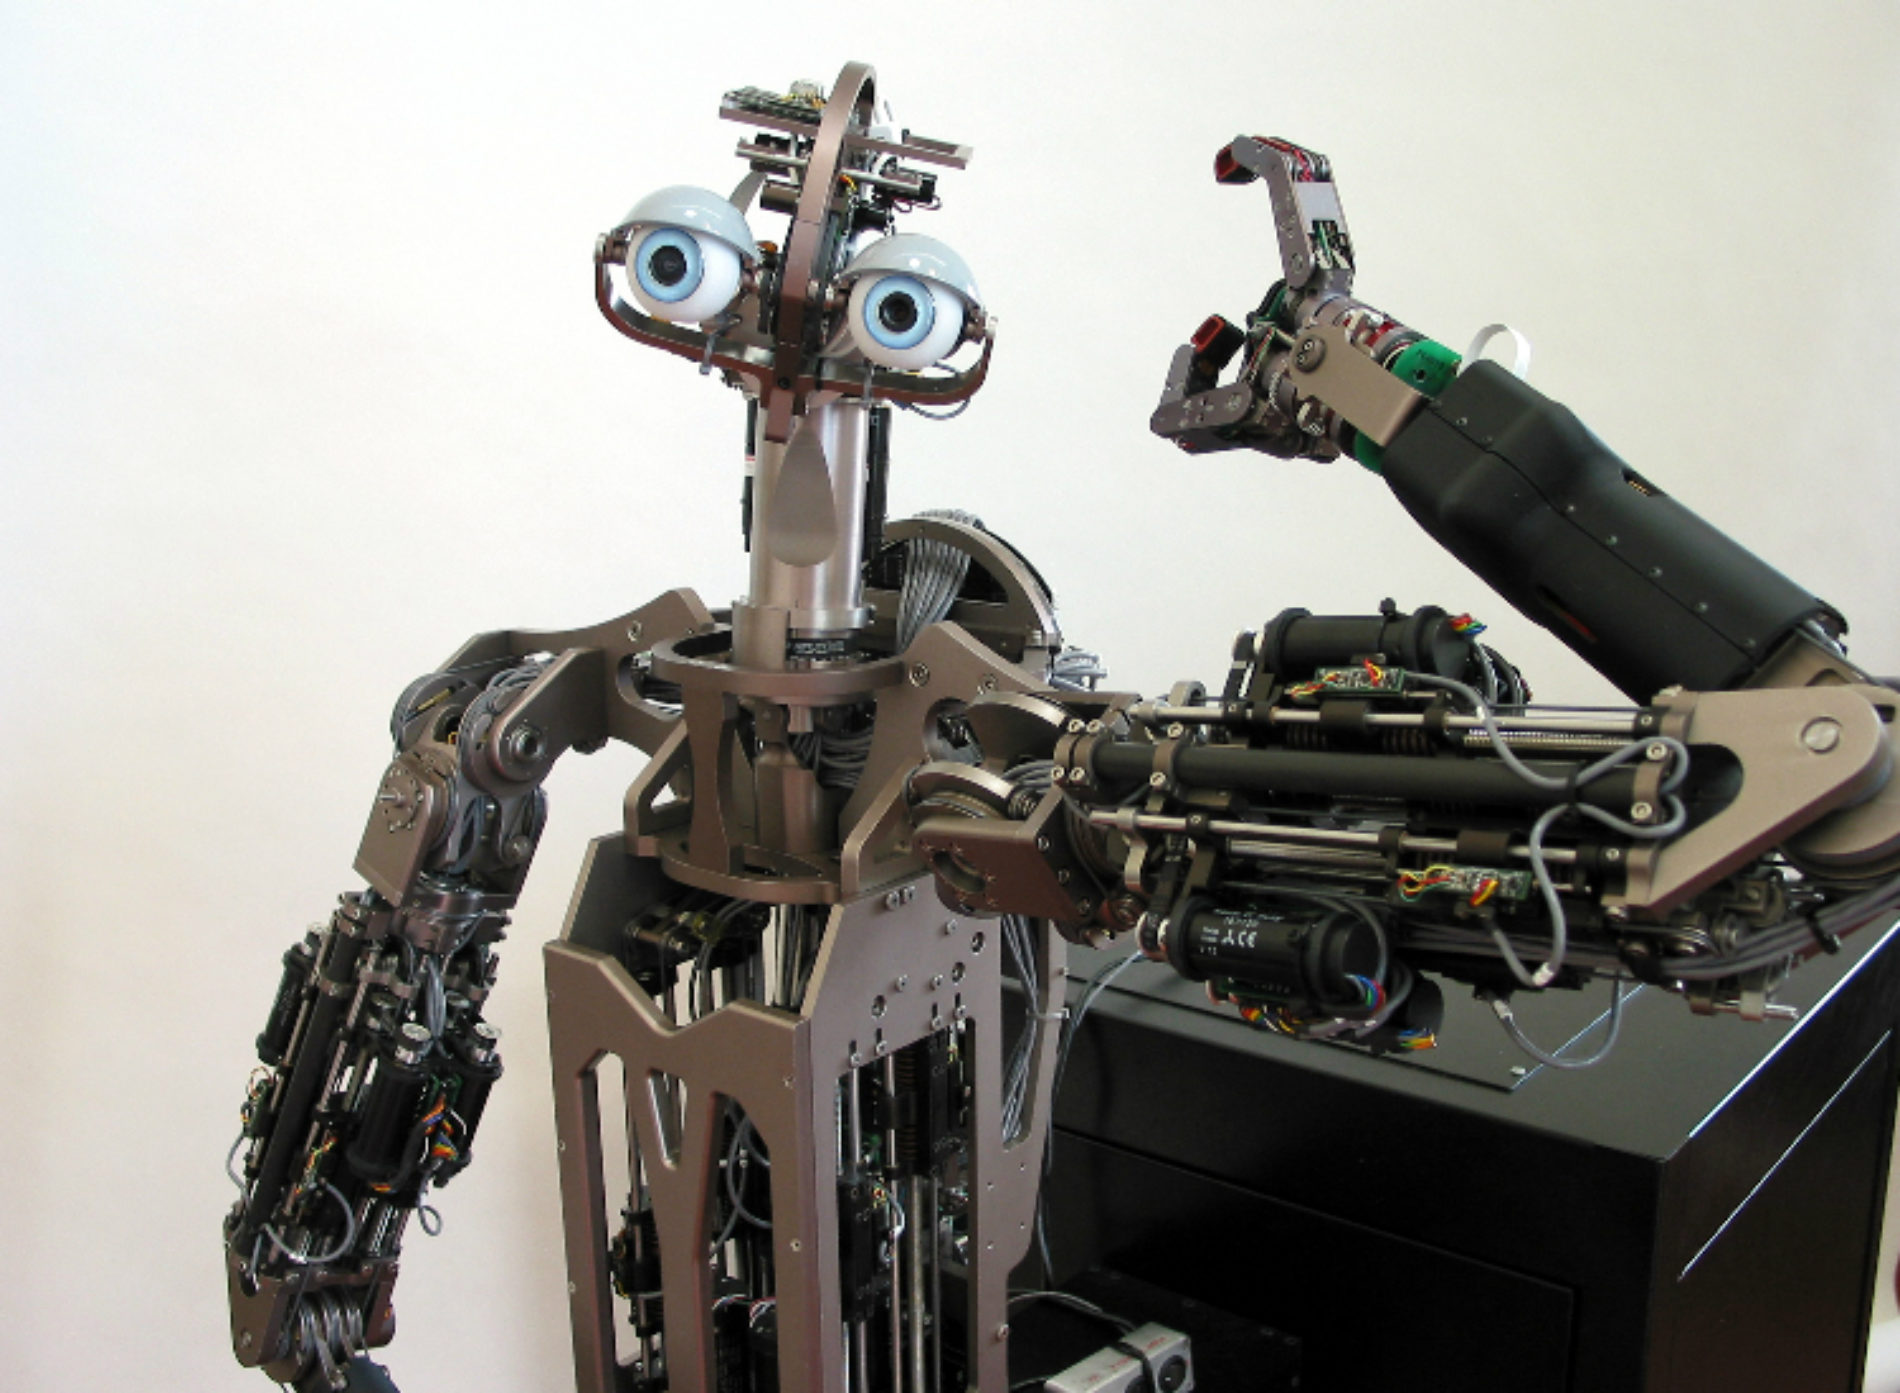
\includegraphics[width=0.6\linewidth]{tex/figs/domo-foto.jpg}
    \caption{Foto Robô Domo (Fonte: http://www.robotsvoice.com)}
    \label{fig:domorobot}
\end{figure}

Anos depois, os mesmos conceitos foram incorporados no robô Meka, figura \ref{fig:meka}, surgido como produto da empresa Meka Robotics fundada por Aaron e Jeff em 2006. Como pode ser notado pelas similaridades do ombro e design do braço em relação a figura \ref{fig:domorobot}. Este robô foi adquirido pelo LARA, porém em 2013 a empresa é adquirida pela Google e toda a documentação do Meka foi retirada do ar. 

% Citar OceanOne (Stanford)?

\begin{figure}[H]
    \centering
    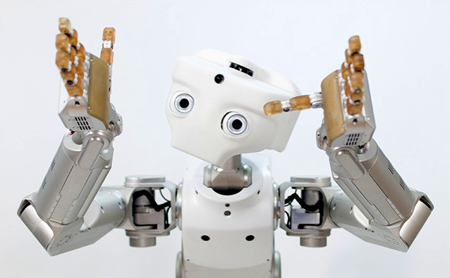
\includegraphics[width=0.6\linewidth]{tex/figs/meka-robot.png}
    \caption{Meka M1 (Fonte: https://spectrum.ieee.org)}
    \label{fig:meka}
\end{figure}

Da mesma linha de trabalhos surgiu a empresa Rethink Robotics fundada por Rodney Brooks, então professor do MIT em 1995. Estes aspectos estudados nos humanoides desenvolvidos no MIT como o COG e o DOMO permitiram que manipuladores robóticos pudessem ter um custo reduzido e atuar com um pouco mais de flexibilidade no ambiente, permitindo a presença de pessoa em proximidade.

% MIT Warehouse
Estes projetos tiveram particular importância pois muitos dos conceitos explorados vieram a compor patentes e futuramente partes dos robôs Baxter (Figura \ref{fig:baxter}) e Meka (Figura \ref{fig:meka}) , respectivamente das empresas Rethink Robotics e Meka Robótics. %Da mesma equipe que desenvolveu o Domo surgiu a Meka Robótics a partir de Aaron Singer e Jeff Weber.
%Bem como dos trabalhos de Pratt e Williason \cite{pratt1995series} surgiu a empresa Rethink Robotics fundada por Rodney Brooks, então professor do MIT em 1995. Estes aspectos estudados permitiram que manipuladores robóticos pudessem ter um custo reduzido e atuar com um pouco mais de flexibilidade no ambiente, permitindo a presença de pessoa em proximidade.

% Baxter vs Meka
Embora com design completamente diferente, o Meka e o Baxter têm como semelhança o uso atuadores série elásticos em cada uma das juntas como elemento de segurança. Desta forma qualquer pessoa pode manusear os braços de ambos robôs além de proteger a estrutura em caso de colisão\cite{pratt1995series}. No entanto este sistema também confere ao robô uma maior suscetibilidade a influência de outros estímulos externos como a ação da gravidade na dinâmica do robô.

\begin{figure}[H]
    \centering
    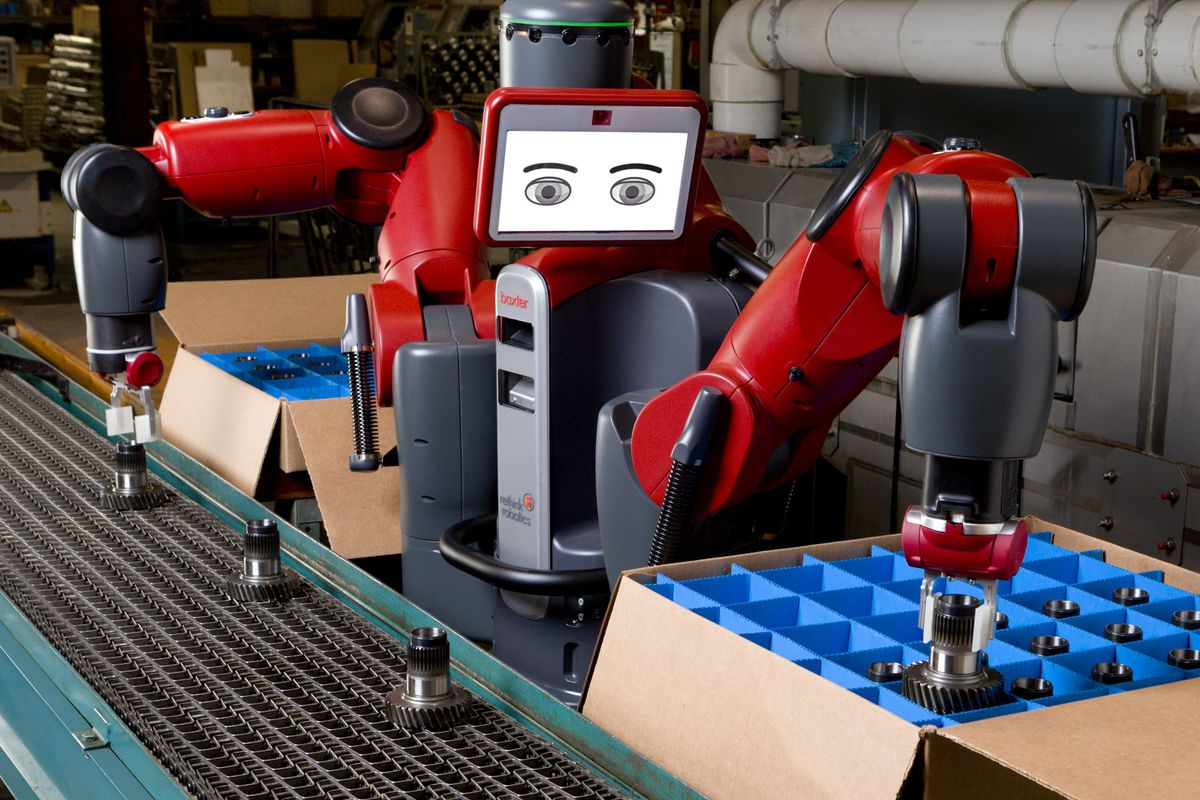
\includegraphics[width = 0.6\linewidth]{tex/figs/baxter_production.jpg}
    \caption{Baxter em linha de produção}
    \label{fig:baxter}
\end{figure}

A compensação da gravidade é resolvido de forma diferente em cada uma das plataformas. No Baxter a compensação da gravidade é feita por compensação mecânica por uma série de molas e via software através do modelo dinâmico em conjunto da biblioteca Orocos KDL\cite{baxterguide}. E no Meka esta é feita apenas por software pela KDL.\cite{mekaguide}

% Robonauta -> Paradigmas atuais

\section{Definição do problema}

No Laboratório de Automação e Robótica ( LARA - UnB ) encontra-se disponível o braço robótico Meka A2 fornecido pela Meka Robotics. Daqui em diante será denominado apenas Meka. O Meka é um braço complacente antropomórfico composto por sete juntas e uma garra desenvolvido para pesquisas na área de interação com pessoas. Em trabalhos anteriores do LARA \cite{marcosps2016} e \cite{koji2017} foi observado um desempenho ineficiente nos controles cinemáticos implementados em contraste ao resultado observado em outras plataformas robóticas e em simulação. Tal arquitetura não encontra-se devidamente documentada e detalhada. Desta forma, neste trabalho, propõe-se realizar uma caracterização mais detalhada desta arquitetura de controle para compreender sua implicação no desempenho dos controles cinemáticos testados e propor melhorias que resultem em trajetórias mais precisas levando em conta as características próprias do sistema.

% Foto Meka
\begin{figure}[H]
    \centering
    \includegraphics[width=0.6\linewidth]{figs/meka}
    \caption{Braço Robótico Meka A2 disponível no Lara \cite{marcosps2016}}
    \label{fig:meka_arm}
\end{figure}

\section{Metodologia}

% Rever completamente N
Este trabalho foi desenvolvido em três etapas: estudo sobre teoria clássica de controle de manipuladores, revisão e acompanhamento de trabalhos anteriores feitos no LARA utilizando o Meka e por fim a investigação e experimentação usando a plataforma. Esta investigação foi feita a partir dos métodos de análise e síntese do processo. Por meio da análise foram estudados cada um dos componentes utilizados tanto de hardware como software em seu detalhes. Em conjunto alguns dos fenômenos foram sintetizados por meio de simulações visando ampliar a compreensão de quais fatores ocasionam ao Meka um desempenho inferior outros a braços robóticos avaliados pelos trabalhos de Murilo \cite{murlow2014} e Marcos \cite{marcosps2016}.

\subsection{Revisão trabalhos anteriores}

Inicialmente foi feito um estudo sobre os trabalho anteriores desenvolvidos na plataforma no Laboratório de Automação e Robótica ( LARA - UnB ) bem como estratégias clássicas no controle de robôs industriais. Alguns destes trabalhos puderam ser acompanhados ao longo da execução como o caso dos trabalhos desenvolvidos por Marcos Pereira \cite{marcosps2016} e pelo Rafael Koji \cite{koji2017} de modo a facilitar a transmissão do conhecimento relacionado as contribuições de cada um ao projeto bem como presenciar as dificuldades relacionadas ao controle do braço robótico.

\subsection{Investigação e experimentação a partir da plataforma}

Após o estudo preliminar foi adotado uma metodologia de investigação baseada em ciclos compostos por 3 etapas, descritas a seguir. Estas etapas são baseadas nos princípios de desenvolvimento ágil \footnote{\url{http://agilemanifesto.org}} e têm como objetivo acelerar e otimizar os esforços.

% TODO Colocar Referência

% Diagrama das etapas
\begin{enumerate}
    \item Análise e Formulação de Hipóteses
    \item Formulação de Testes para as Hipóteses
    \item Avaliação de Hipóteses ( Testes Experimentais e Estudo teórico )
\end{enumerate}

Cada ciclo possui duração variável de acordo com o nível de aprofundamento necessário para satisfazer os objetivos levantados para cada momento do projeto. O objetivo central é ao final de um ciclo é trazer algum aprimoramento quanto ao entendimento do sistema ou ainda quanto ao comportamento final na realização da tarefa.

No inicio de cada ciclo é feito um estudo do sistema através da modelagem do sistema e da definição de uma métrica para avaliar o comportamento. Então o comportamento do sistema real é comparado com o modelo adotado e as expectativas de comportamento. Os objetivos são traduzidos em uma métrica, compondo um conjunto de indicadores que permita avaliar se tarefa foi executada e como foi o processo de execução. A cada novo aspecto avaliado podem ser introduzidos novos indicadores em conjunto aos antigos ou modificados. 

Com base nisto são levantadas hipóteses quanto ao comportamento quanto ao fato de satisfazer ou não o modelo adotado e possíveis condutas para aprimorar os resultados dentro da métrica proposta. Para cada uma destas condutas é levantado um teste de verificação que pode incluir consulta bibliográfica, simulações a partir do modelo e experimentos com o Meka. Os resultados desta etapa são então levados para a etapa de observação e confrontados novamente e assim o ciclo se repete.

Resultados positivos são incorporados e resultados negativos avaliados quanto a possíveis correções. Tudo é registrado para permitir futuras avaliações. Como efeito foi feito um registro das atividades e todo material produzido, incluindo registro de dados dos experimentos e scripts usados para processar os dados, foi colocado no GitHub \footnote{www.github.com/lara-unb/Meka} de forma a permitir o uso futuro na validação do comportamento após modificações futuras.

\section{Estrutura do Documento}

Este trabalho está dividido em 5 capítulos visando facilitar o entendimento. Estes estão organizados da seguinte forma:

\begin{itemize}
    \item \textit{Cap. \ref{ch:intro} Introdução} : Breve Apresentação e Histórico sobre Robótica Colaborativa.
    \item \textit{Cap. \ref{ch:teory-reference} Fundamentos} : Conceitos teóricos e tecnologias usadas no trabalho.
    \item \textit{Cap. \ref{ch:develop} Desenvolvimento} : Metodologia usada na investigação dos problemas e análise dos dados.
    \item \textit{Cap. \ref{ch:results} Resultados} : Dados obtidos ao longo do trabalho.
    \item \textit{Cap. \ref{ch:conclusoes} Conclusão} : Resultado final do trabalho e propostas de trabalhos futuros.
\end{itemize}
